\documentclass[a4paper,12pt,titlepage]{article}
\usepackage{amsmath} 
\usepackage{amssymb}
\usepackage[nottoc]{tocbibind}
\usepackage{float}
\usepackage{indentfirst}
\author{\textit{Jiang Yicheng}\\\textit{515370910224}}
\title{\textbf{VV286\\ Honors Mathematics IV\\
Ordinary Differential Equations\\
		Assignment 7}}
\date{\today}
\usepackage{extarrows}
\usepackage{mathrsfs}
\usepackage{dsfont}
\usepackage[top=1 in, bottom=0.8 in, left= 1in, right=1 in]{geometry}
\usepackage{fancyhdr,lastpage}
	\pagestyle{fancy}
	\fancyhf{}
\cfoot{Page \thepage\ of \pageref{LastPage}}
\usepackage{multirow}
\usepackage{gauss}
\usepackage{geometry}
\usepackage{graphicx}
\begin{document}

\maketitle

\section*{Exercise 7.1}
$\forall k\in\mathbb{N}$, 
\begin{align*}
&\int_{kT}^{kT+T}f(t)e^{-pt}dt\xlongequal {s=t-kT}\int_{0}^{T}f(s+kT)e^{-p(s+kT)}ds=e^{-pkT}\int_{0}^{T}f(s)e^{-ps}ds
\end{align*}
Then 
\begin{align*}
(\mathcal{L}f)(p)&=\int_{0}^{\infty}f(t)e^{-pt}dt=\sum\limits_{k=0}^{\infty}e^{-pkT}\int_{0}^{T}f(s)e^{-ps}ds=\int_{0}^{T}f(s)e^{-ps}ds\underset{k\rightarrow \infty}{lim}\dfrac{1-e^{-pT(k+1)}}{1-e^{-pT}}\\
&\xlongequal {p>0}\dfrac{1}{1-e^{-pT}}\int_{0}^{T}f(s)e^{-ps}ds
\end{align*}
So $(\mathcal{L}f)(p)=\dfrac{1}{1-e^{-pT}}\int_{0}^{T}f(s)e^{-ps}ds$.

Then for $f(t)=at,t\in[0,1]$ with period $T=1$,
\begin{align*}
(\mathcal{L}f)(p)&=\dfrac{1}{1-e^{-pT}}\int_{0}^{T}f(t)e^{-pt}dt=\dfrac{1}{1-e^{-p}}\int_{0}^{1}ate^{-pt}dt\\
&=\dfrac{1}{1-e^{-p}}a\Big(-\dfrac{1}{p}(t+\dfrac{1}{p})e^{-pt}|_{0}^{1}\Big)\\
&=\dfrac{1}{1-e^{-p}}a\Big(-\dfrac{1}{p}(1+\dfrac{1}{p})e^{-p}+\dfrac{1}{p}(0+\dfrac{1}{p})\Big)\\
&=\dfrac{a(1-(p+1)e^{-p})}{p^2(1-e^{-p})}
\end{align*}

So the Laplace transform of the function
$$f(t) = at, a \in \mathbb{R}, t \in [0, 1]$$
is $(\mathcal{L}f)(p)=\dfrac{a(1-(p+1)e^{-p})}{p^2(1-e^{-p})}$.

\section*{Exercise 7.2}
\subsection*{i)}
For $F(p)=\dfrac{1}{p(e^p+1)}$, 
\begin{align*}
(\mathcal{M}F)(t)=\dfrac{1}{2\pi i}\int_{\beta-i\infty}^{\beta+i\infty}e^{pt}\dfrac{1}{p(e^p+1)}dp
\end{align*}
Since
\begin{align*}
\underset{\pi/2\leqslant\theta\leqslant3\pi/2}{sup}|F(Re^{i\theta})|&=\underset{\pi/2\leqslant\theta\leqslant3\pi/2}{sup}|\dfrac{1}{Re^{i\theta}(e^{Re^{i\theta}}+1)}|\\
&=\dfrac{1}{R}\underset{\pi/2\leqslant\theta\leqslant3\pi/2}{sup}|\dfrac{1}{e^{R\cos\theta}(\cos(R\sin\theta)+i\sin(R\sin\theta))+1}|\\
&=\dfrac{1}{R}\underset{\pi/2\leqslant\theta\leqslant3\pi/2}{sup}\dfrac{1}{\sqrt{1+e^{2R\cos\theta}+2e^{R\cos\theta}\cos(R\sin\theta)}}\\
&\xlongequal{R\rightarrow\infty} O(\dfrac{1}{R})
\end{align*}
we can apply Jordan's Lemma and obtain that
$$(\mathcal{M}F)(t)=\dfrac{1}{2\pi i}\int_{\beta-i\infty}^{\beta+i\infty}e^{pt}\dfrac{1}{p(e^p+1)}dp=\sum\limits_{k=-\infty}^{\infty}res_{p_k}e^{pt}F(p)$$
where $p_k$ is the pole of $e^{pt}F(p)$ with $p_0=0,p_k=i(2k+1)\pi$ and 
\begin{align*}
res_{p_k}e^{pt}F(p)&=\underset{p\rightarrow i(2k+1)\pi}{lim}(p-i(2k+1)\pi)\dfrac{e^{pt}}{p(e^p+1)}=-\dfrac{e^{i(2k+1)\pi t}}{i(2k+1)\pi}\\
&=\dfrac{\cos((2k+1)\pi t)+i\sin((2k+1)\pi t)}{(2k+1)\pi}i\\
res_{p_0}e^{pt}F(p)&=\underset{p\rightarrow 0}{lim}(p-0)\dfrac{e^{pt}}{p(e^p+1)}=\dfrac{1}{2}
\end{align*}
So
\begin{align*}
(\mathcal{M}F)(t)&=Re(\sum\limits_{k=-\infty}^{\infty}res_{p_k}e^{pt}F(p))\\
&=\dfrac{1}{2}-\sum\limits_{k=-\infty}^{\infty}\dfrac{\sin((2k+1)\pi t)}{(2k+1)\pi}=\dfrac{1}{2}-\dfrac{2}{\pi}\sum\limits_{k=0}^{\infty}\dfrac{\sin((2k+1)\pi t)}{2k+1}\\
&=\dfrac{1}{2}-\dfrac{2}{\pi}(\sin(\pi t)+\dfrac{\sin(3\pi t)}{3}+\dfrac{\sin(5\pi t)}{5}+\cdots)
\end{align*}
So
$$(\mathcal{L}^{-1}F)(t)=\dfrac{1}{2}-\dfrac{2}{\pi}(\sin(\pi t)+\dfrac{\sin(3\pi t)}{3}+\dfrac{\sin(5\pi t)}{5}+\cdots)$$

\subsection*{ii)}
For $F(p)=\dfrac{1}{p\cosh p}$, 
\begin{align*}
(\mathcal{M}F)(t)=\dfrac{1}{2\pi i}\int_{\beta-i\infty}^{\beta+i\infty}e^{pt}\dfrac{1}{p\cosh p}dp
\end{align*}
Since
\begin{align*}
\underset{\pi/2\leqslant\theta\leqslant3\pi/2}{sup}|F(Re^{i\theta})|&=\underset{\pi/2\leqslant\theta\leqslant3\pi/2}{sup}|\dfrac{1}{Re^{i\theta}\cosh (Re^{i\theta})}|\xlongequal{R\rightarrow\infty} O(\dfrac{1}{R})
\end{align*}
we can apply Jordan's Lemma and obtain that
$$(\mathcal{M}F)(t)=\dfrac{1}{2\pi i}\int_{\beta-i\infty}^{\beta+i\infty}e^{pt}\dfrac{1}{p\cosh p}dp=\sum\limits_{k=-\infty}^{\infty}res_{p_k}e^{pt}F(p)$$
where $p_k$ is the pole of $e^{pt}F(p)$ with $p_0=0,p_k=i(2k+1)\pi/2$ and 
\begin{align*}
res_{p_k}e^{pt}F(p)&=\underset{p\rightarrow i(2k+1)\pi/2}{lim}(p-i(2k+1)\pi/2)\dfrac{e^{pt}}{p\cosh p}=\dfrac{e^{i(2k+1)\pi t}}{i(2k+1)\pi/2\sinh (i(2k+1)\pi/2)}\\
&=\dfrac{2(-1)^{k+1}(\cos((2k+1)\pi/2 t)+i\sin((2k+1)\pi/2 t))}{(2k+1)\pi}\\
res_{p_0}e^{pt}F(p)&=\underset{p\rightarrow 0}{lim}(p-0)\dfrac{e^{pt}}{p\cosh p}=\dfrac{1}{2}
\end{align*}
So
\begin{align*}
(\mathcal{M}F)(t)&=Re(\sum\limits_{k=-\infty}^{\infty}res_{p_k}e^{pt}F(p))\\
&=\dfrac{1}{2}-2\sum\limits_{k=-\infty}^{\infty}(-1)^{k}\dfrac{\cos((2k+1)\pi/2 t)}{(2k+1)\pi}=\dfrac{1}{2}-\dfrac{4}{\pi}\sum\limits_{k=0}^{\infty}\dfrac{\cos((2k+1)\pi/2 t)}{2k+1}\\
&=\dfrac{1}{2}-\dfrac{4}{\pi}(\cos(\pi/2 t)-\dfrac{\cos(3\pi/2 t)}{3}+\dfrac{\cos(5\pi/2 t)}{5}+\cdots)
\end{align*}
So
$$(\mathcal{L}^{-1}F)(t)=\dfrac{1}{2}-\dfrac{4}{\pi}(\cos(\dfrac{\pi}{2} t)-\dfrac{1}{3}\cos(\dfrac{3\pi}{2} t)+\cdots)$$

\section*{Exercise 7.3}
For $f(t)=\left\{
\begin{aligned}
2,0\leqslant t\leqslant1\\
0,1\leqslant t\leqslant2\\
\end{aligned}
\right.
$ with period $T=2$,
\begin{align*}
(\mathcal{L}f)(p)&=\dfrac{1}{1-e^{-pT}}\int_{0}^{T}f(t)e^{-pt}dt=\dfrac{1}{1-e^{-2p}}\Big(\int_{0}^{1}2e^{-pt}dt+\int_1^20\cdot e^{-pt}dt\Big)\\
&=\dfrac{1}{1-e^{-2p}}\Big(-\dfrac{2}{p}e^{-pt}|_{0}^{1}\Big)\\
&=\dfrac{1}{1-e^{-2p}}\Big(-\dfrac{2}{p}(e^{-p}-1)\Big)\\
&=\dfrac{2(1-e^{-p})}{p(1-e^{-2p})}=\dfrac{2}{p(1+e^{-p})}\\
&=\dfrac{(e^{p/2}+e^{-p/2})+(e^{p/2}-e^{-p/2})}{p(e^{p/2}+e^{-p/2})}\\
&=\dfrac{1+\tanh(p/2)}{p}
\end{align*}

So the Laplace transform of the function
is $(\mathcal{L}f)(p)=\dfrac{1+\tanh(p/2)}{p}$.

For $F(p)=\dfrac{1+\tanh(p/2)}{p}$, 
\begin{align*}
(\mathcal{M}F)(t)=\dfrac{1}{2\pi i}\int_{\beta-i\infty}^{\beta+i\infty}e^{pt}\dfrac{1+\tanh(p/2)}{p}dp
\end{align*}
Since
\begin{align*}
\underset{\pi/2\leqslant\theta\leqslant3\pi/2}{sup}|F(Re^{i\theta})|&=\underset{\pi/2\leqslant\theta\leqslant3\pi/2}{sup}|\dfrac{1+\tanh(Re^{i\theta}/2)}{Re^{i\theta}}|\xlongequal{R\rightarrow\infty} O(\dfrac{1}{R})
\end{align*}
we can apply Jordan's Lemma and obtain that
$$(\mathcal{M}F)(t)=\dfrac{1}{2\pi i}\int_{\beta-i\infty}^{\beta+i\infty}e^{pt}\dfrac{2}{p(1+e^{-p})}dp=\sum\limits_{k=-\infty}^{\infty}res_{p_k}e^{pt}F(p)$$
where $p_k$ is the pole of $e^{pt}F(p)$ with $p_0=0,p_k=i(2k+1)\pi$ and 
\begin{align*}
res_{p_k}e^{pt}F(p)&=\underset{p\rightarrow i(2k+1)\pi}{lim}(p-i(2k+1)\pi)\dfrac{2e^{pt}}{p(e^{-p}+1)}=\dfrac{2e^{i(2k+1)\pi t}}{i(2k+1)\pi}\\
&=-2\dfrac{\cos((2k+1)\pi t)+i\sin((2k+1)\pi t)}{(2k+1)\pi}i\\
res_{p_0}e^{pt}F(p)&=\underset{p\rightarrow 0}{lim}(p-0)\dfrac{2e^{pt}}{p(e^{-p}+1)}=1
\end{align*}
So
\begin{align*}
(\mathcal{M}F)(t)&=Re(\sum\limits_{k=-\infty}^{\infty}res_{p_k}e^{pt}F(p))\\
&=1+2\sum\limits_{k=-\infty}^{\infty}\dfrac{\sin((2k+1)\pi t)}{(2k+1)\pi}\\
&=1+\dfrac{4}{\pi}\sum\limits_{k=0}^{\infty}\dfrac{\sin((2k+1)\pi t)}{2k+1}
\end{align*}

\begin{figure}[H]
    \centering
    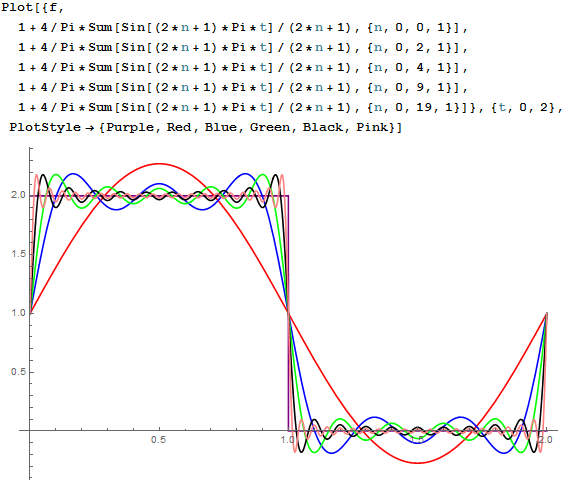
\includegraphics[scale=1]{0.png}
    \caption{Function $f$ (purple) together with $n = 1$ (red), 3 (blue), 5 (green), 10 (black), 20 (pink) terms of the series $(\mathcal{M}F)(t)=1+\dfrac{4}{\pi}\sum\limits_{k=0}^{\infty}\dfrac{\sin((2k+1)\pi t)}{2k+1}$.}
\end{figure}

\section*{Exercise 7.4}
\subsection*{i)$y''+y=\sin t+\delta(t-\pi),y(0)=0,y'(0)=0$}
Set $Y(p)=(\mathcal{L}y)(p)$, then
$$(\mathcal{L}y')(p)=p\cdot(\mathcal{L}y)(p)-y(0)=pY(p) $$
$$(\mathcal{L}y'')(p)=p\cdot(\mathcal{L}y')(p)-y'(0)=p^2Y(p) $$

and
$$\Big(\mathcal{L}(\sin t+\delta(t-\pi))\Big)(p)=\dfrac{1}{p^2+1}+e^{-\pi p}$$
So apply Laplace transform to the equation and we get
\begin{align*}
&(p^2+1)Y(p)=\dfrac{1}{p^2+1}+e^{-\pi p}\\
\Rightarrow& Y(p)=\dfrac{1}{p^2+1}\dfrac{1}{p^2+1}+e^{-\pi p}\dfrac{1}{p^2+1}\\
\Rightarrow& Y(p)=\mathcal{L}(\sin t)\mathcal{L}(\sin t)+e^{-\pi p}(\mathcal{L}(\sin t))
\end{align*}
Since
\begin{align*}
&\sin t*\sin t\\
=&\int_0^t \sin (t-s)\sin sds =\dfrac{1}{2}\int_0^t \cos(t-2s)-\cos tds\\
=&\dfrac{1}{2}(\dfrac{1}{2}\sin(2s-t)-s\cos t)\Big|_{0}^{t}    \\
=&\dfrac{1}{2}(\sin t-t\cos t)
\end{align*}
Then 
\begin{align*}
(\mathcal{L}^{-1}Y)(t)=\dfrac{1}{2}(\sin t-t\cos t)+\sin(t-\pi)H(t-\pi)
\end{align*}
So the solution to the equation is $y(t)=\dfrac{1}{2}(\sin t-t\cos t)+\sin(t-\pi)H(t-\pi)$

\subsection*{ii)$y''+y'+y=2\delta (t-1)-\delta(t-2),y(0)=1,y'(0)=0$}
Set $Y(p)=(\mathcal{L}y)(p)$, then
$$(\mathcal{L}y')(p)=p\cdot(\mathcal{L}y)(p)-y(0)=pY(p)-1 $$
$$(\mathcal{L}y'')(p)=p\cdot(\mathcal{L}y')(p)-y'(0)=p^2Y(p)-p $$
and
$$\Big(\mathcal{L}(2\delta (t-1)-\delta(t-2))\Big)(p)=2e^{-p}-e^{-2 p}$$
So apply Laplace transform to the equation and we get
\begin{align*}
&(p^2+p+1)Y(p)=2e^{-p}-e^{-2 p}+p+1\Rightarrow Y(p)=\dfrac{2e^{-p}}{p^2+p+1}+\dfrac{p+1}{p^2+p+1}\\
\Rightarrow& Y(p)=\dfrac{4}{\sqrt{3}}e^{-p}\dfrac{\frac{\sqrt{3}}{2}}{(p+\frac{1}{2})^2+(\frac{\sqrt{3}}{2})^2}+\dfrac{p+\frac{1}{2}}{(p+\frac{1}{2})^2+(\frac{\sqrt{3}}{2})^2}+\dfrac{1}{\sqrt{3}}\dfrac{\frac{\sqrt{3}}{2}}{(p+\frac{1}{2})^2+(\frac{\sqrt{3}}{2})^2}
\end{align*}

Then 
\begin{align*}
(\mathcal{L}^{-1}Y)(t)&=\dfrac{4}{\sqrt{3}}(\mathcal{L}^{-1}e^{-p}e^{-\frac{1}{2}t}\sin \frac{\sqrt{3}}{2}t)+e^{-\frac{1}{2}t}\cos \frac{\sqrt{3}}{2}t+\dfrac{1}{\sqrt{3}}e^{-\frac{1}{2}t}\sin \frac{\sqrt{3}}{2}t\\
&=\dfrac{4}{\sqrt{3}}e^{-\frac{1}{2}(t-1)}\sin \frac{\sqrt{3}}{2}(t-1)H(t-1)+\dfrac{2e^{-\frac{1}{2}t}}{\sqrt{3}}\sin (\frac{\sqrt{3}}{2}t+\dfrac{\pi}{3})
\end{align*}
So the solution to the equation is $$y(t)=\dfrac{4}{\sqrt{3}}e^{-\frac{1}{2}(t-1)}\sin \frac{\sqrt{3}}{2}(t-1)H(t-1)+\dfrac{2e^{-\frac{1}{2}t}}{\sqrt{3}}\sin (\frac{\sqrt{3}}{2}t+\frac{\pi}{3})$$

\section*{Exercise 7.5}
\subsection*{i)$ \dfrac{d^2y}{dt^2}+y=\sum\limits_{j=0}^{\infty}\delta(t-j\pi),y(0)=y'(0)=0 $}
Set $Y(p)=(\mathcal{L}y)(p)$, then
$$(\mathcal{L}y')(p)=p\cdot(\mathcal{L}y)(p)-y(0)=pY(p) $$
$$(\mathcal{L}y'')(p)=p\cdot(\mathcal{L}y')(p)-y'(0)=p^2Y(p) $$

and
$$\Big(\mathcal{L}(\sum\limits_{j=0}^{\infty}\delta(t-j\pi))\Big)(p)=\sum\limits_{j=0}^{\infty}e^{-j\pi p}=\dfrac{1}{1-e^{-\pi p}},p>0$$
So apply Laplace transform to the equation and we get
\begin{align*}
&(p^2+1)Y(p)=\sum\limits_{j=0}^{\infty}e^{-j\pi p}\Rightarrow Y(p)=\sum\limits_{j=0}^{\infty}e^{-j\pi p}\dfrac{1}{p^2+1}\\
\Rightarrow& \mathcal{L}^{-1}(Y(p))=\sum\limits_{j=0}^{\infty}\sin (t-j\pi)H(t-j\pi)
\end{align*}
Since
\begin{align*}
\sin (t-j\pi)H(t-j\pi)=\left\{
\begin{aligned}
&(-1)^j\sin t,t\geqslant j\pi\\
&0,s<j\pi\\
\end{aligned}
\right.
\end{align*}
then for  $n$ is even, $\forall t\in n\pi<t<(n+1)\pi$ 
\begin{align*}
\sum\limits_{j=0}^{\infty}\sin (t-j\pi)H(t-j\pi)=\sum\limits_{j=0}^{n}(-1)^{j}\sin t=\sin t
\end{align*}
and for  $n$ is odd, $\forall t\in n\pi<t<(n+1)\pi$ 
\begin{align*}
\sum\limits_{j=0}^{\infty}\sin (t-j\pi)H(t-j\pi)=\sum\limits_{j=0}^{n}(-1)^{j}\sin t=0
\end{align*}
So the solution to the equation is $$y(t)=\left\{
\begin{aligned}
&\sin t,n\,\,is\,\,even\\
&0\,\,\,\,\,\,\,\,,n\,\,is\,\,odd\\
\end{aligned}
\right.$$
for $ t\in n\pi<t<(n+1)\pi$

\subsection*{ii)$ \dfrac{d^2y}{dt^2}+y=\sum\limits_{j=0}^{\infty}\delta(t-2j\pi),y(0)=y'(0)=0 $}
Set $Y(p)=(\mathcal{L}y)(p)$, then
$$(\mathcal{L}y')(p)=p\cdot(\mathcal{L}y)(p)-y(0)=pY(p) $$
$$(\mathcal{L}y'')(p)=p\cdot(\mathcal{L}y')(p)-y'(0)=p^2Y(p) $$

and
$$\Big(\mathcal{L}(\sum\limits_{j=0}^{\infty}\delta(t-2j\pi))\Big)(p)=\sum\limits_{j=0}^{\infty}e^{-2j\pi p}=\dfrac{1}{1-e^{-2\pi p}},p>0$$
So apply Laplace transform to the equation and we get
\begin{align*}
&(p^2+1)Y(p)=\sum\limits_{j=0}^{\infty}e^{-2j\pi p}\Rightarrow Y(p)=\sum\limits_{j=0}^{\infty}e^{-2j\pi p}\dfrac{1}{p^2+1}\\
\Rightarrow& \mathcal{L}^{-1}(Y(p))=\sum\limits_{j=0}^{\infty}\sin (t-2j\pi)H(t-2j\pi)=\sum\limits_{j=0}^{\infty}\sin tH(t-2j\pi)
\end{align*}
Since
\begin{align*}
\sin tH(t-2j\pi)=\left\{
\begin{aligned}
&\sin t,t\geqslant 2j\pi\\
&0,s<2j\pi\\
\end{aligned}
\right.
\end{align*}
then $\forall t\in 2n\pi<t<2(n+1)\pi$ 
\begin{align*}
\sum\limits_{j=0}^{\infty}\sin tH(t-2j\pi)=\sum\limits_{j=0}^{n}\sin t=(n+1)\sin t
\end{align*}

So the solution to the equation is $$y(t)=(n+1)\sin t$$
for $ t\in 2n\pi<t<2(n+1)\pi$


\section*{Exercise 7.6}
\subsection*{i)}
For $\Pi(x)=\left\{
\begin{aligned}
1,|x|<1\\
0,|x|\geqslant1\\
\end{aligned}
\right.$, we have that
\begin{align*}
(\widehat{\Pi})(\xi)&=\dfrac{1}{\sqrt{2\pi}}\int_{-\infty}^{\infty}\Pi(x)e^{-i\xi x}dx=\dfrac{1}{\sqrt{2\pi}}\int_{-1}^{1}e^{-i\xi x}dx\\
&=\dfrac{1}{\sqrt{2\pi}}\dfrac{1}{-i\xi}e^{-i\xi x}\Big|_{-1}^1=\sqrt{\dfrac{2}{\pi}}\dfrac{\sin\xi}{\xi}
\end{align*}
So $(\widehat{\Pi})(\xi)=\sqrt{\dfrac{2}{\pi}}\dfrac{\sin\xi}{\xi}$.

\subsection*{ii)}
In the former assignment, we have proved that $$\int_{-\infty}^{\infty}\dfrac{e^{iz}-1}{2iz}=\dfrac{\pi}{2}$$
and for $x\neq\pm1$
$$\dfrac{e^{ix\xi}\sin\xi}{\xi}=-(x-1)\dfrac{e^{i(x-1)\xi}-1}{2i(x-1)\xi}+(x+1)\dfrac{e^{i(x+1)\xi
}-1}{2i(x+1)\xi})$$ 
so if $x<-1$
\begin{align*}
&\dfrac{1}{\sqrt{2\pi}}\int_{-\infty}^{\infty}\sqrt{\dfrac{2}{\pi}}\dfrac{e^{ix\xi}\sin\xi}{\xi}d\xi\\
=&\dfrac{1}{\pi}\int_{-\infty}^{\infty}-(x-1)\dfrac{e^{i(x-1)\xi}-1}{2i(x-1)\xi}+(x+1)\dfrac{e^{i(x+1)\xi
}-1}{2i(x+1)\xi})d\xi\\
=&\dfrac{1-x}{\pi(x-1)}\int_{\infty}^{-\infty}\dfrac{e^{iz}-1}{2iz}dz+\dfrac{1+x}{\pi(x+1)}\int_{\infty}^{-\infty}\dfrac{e^{iz}-1}{2iz}dz\\
=&-\dfrac{1}{\pi}\cdot\Big(-\dfrac{\pi}{2}\Big)+\dfrac{1}{\pi}\cdot\Big(-\dfrac{\pi}{2}\Big)\\
=&0
\end{align*}
if $-1<x<1$
\begin{align*}
&\dfrac{1}{\sqrt{2\pi}}\int_{-\infty}^{\infty}\sqrt{\dfrac{2}{\pi}}\dfrac{e^{ix\xi}\sin\xi}{\xi}d\xi\\
=&\dfrac{1}{\pi}\int_{-\infty}^{\infty}-(x-1)\dfrac{e^{i(x-1)\xi}-1}{2i(x-1)\xi}+(x+1)\dfrac{e^{i(x+1)\xi
}-1}{2i(x+1)\xi})d\xi\\
=&\dfrac{1-x}{\pi(x-1)}\int_{\infty}^{-\infty}\dfrac{e^{iz}-1}{2iz}dz+\dfrac{1+x}{\pi(x+1)}\int_{-\infty}^{\infty}\dfrac{e^{iz}-1}{2iz}dz\\
=&-\dfrac{1}{\pi}\cdot\Big(-\dfrac{\pi}{2}\Big)+\dfrac{1}{\pi}\cdot\Big(\dfrac{\pi}{2}\Big)\\
=&1
\end{align*}
if $x>1$
\begin{align*}
&\dfrac{1}{\sqrt{2\pi}}\int_{-\infty}^{\infty}\sqrt{\dfrac{2}{\pi}}\dfrac{e^{ix\xi}\sin\xi}{\xi}d\xi\\
=&\dfrac{1}{\pi}\int_{-\infty}^{\infty}-(x-1)\dfrac{e^{i(x-1)\xi}-1}{2i(x-1)\xi}+(x+1)\dfrac{e^{i(x+1)\xi
}-1}{2i(x+1)\xi})d\xi\\
=&\dfrac{1-x}{\pi(x-1)}\int_{-\infty}^{\infty}\dfrac{e^{iz}-1}{2iz}dz+\dfrac{1+x}{\pi(x+1)}\int_{-\infty}^{\infty}\dfrac{e^{iz}-1}{2iz}dz\\
=&-\dfrac{1}{\pi}\cdot\Big(\dfrac{\pi}{2}\Big)+\dfrac{1}{\pi}\cdot\Big(\dfrac{\pi}{2}\Big)\\
=&0
\end{align*}
if $x=1$
\begin{align*}
&\dfrac{1}{\sqrt{2\pi}}\int_{-\infty}^{\infty}\sqrt{\dfrac{2}{\pi}}\dfrac{e^{i\xi}\sin\xi}{\xi}d\xi\\
=&\dfrac{1}{\pi}\int_{-\infty}^{\infty}\dfrac{e^{i\xi}\sin\xi-1}{\xi}+\dfrac{1}{\xi}d\xi\\
=&\dfrac{1}{\pi}\cdot\dfrac{\pi}{2}+0\\
=&\dfrac{1}{2}
\end{align*}
if $x=-1$
\begin{align*}
&\dfrac{1}{\sqrt{2\pi}}\int_{-\infty}^{\infty}\sqrt{\dfrac{2}{\pi}}\dfrac{e^{i(-\xi)}\sin\xi}{\xi}d\xi\\
=&\dfrac{1}{\pi}\int_{-\infty}^{\infty}\dfrac{e^{i(-\xi)}\sin(-\xi)-1}{-\xi}+\dfrac{1}{\xi}d\xi\\
=&-\dfrac{1}{\pi}\int_{\infty}^{-\infty}\dfrac{e^{iz}\sin z-1}{z}+0\\
=&\dfrac{1}{2}
\end{align*}

To sum up,
$$\dfrac{1}{\sqrt{2\pi}}\int_{-\infty}^{\infty}e^{i\xi}\widehat{\Pi}(\xi)d\xi=\left\{
\begin{aligned}
1,|x|<1\\
\frac{1}{2},|x|=1\\
0,|x|>1
\end{aligned}
\right.$$


\section*{Exercise 7.7}

\begin{align*}
\widehat{f}(\xi+i\eta)=&\dfrac{1}{\sqrt{2\pi}}\int_{-\infty}^{\infty}H(x)x^2e^{-i(\xi+i\eta)x}dx\\
=&\dfrac{1}{\sqrt{2\pi}}\int_{0}^{\infty}x^2e^{-i(\xi+i\eta)x}dx\\
=&\dfrac{1}{\sqrt{2\pi}}\Big(\dfrac{1}{-i(\xi+i\eta)}x^2-\dfrac{1}{(-i(\xi+i\eta))^2}x+\dfrac{2}{(-i(\xi+i\eta))^3}\Big)e^{-i(\xi+i\eta)x}|_{0}^{\infty}
\end{align*}
To make the integral convergent, $e^{-i(\xi+i\eta)x}\xrightarrow{x\rightarrow\infty}0$. So $\eta<0$ i.e. in the region below the real axis in complex plane $\widehat{f}$ defined and
$$\widehat{f}(\xi+i\eta)=0-\dfrac{1}{\sqrt{2\pi}}\dfrac{2}{(-i(\xi+i\eta))^3}=\sqrt{\dfrac{2}{\pi}}\dfrac{1}{(\xi+i\eta))^3}i$$









\end{document}
